\documentclass[tikz,border=10pt]{standalone}
\usepackage{tikz}
\usetikzlibrary{arrows.meta, positioning, fadings, shapes.arrows}

\begin{document}
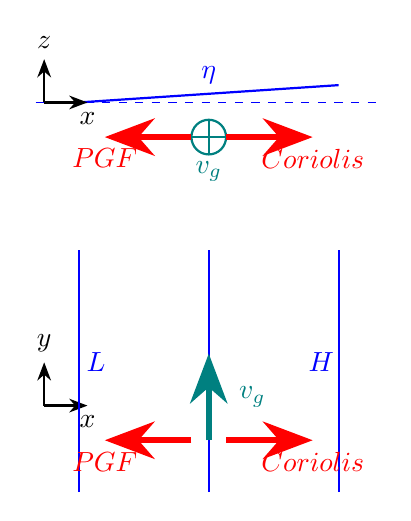
\begin{tikzpicture}[scale=1.1, >=Stealth]

% draw a sea surface height $\eta$ that tilts up to the right:

\draw[thick, blue] (0,0) -- (3,0.2) node[midway, above] {$\eta$};
%draw a dashed line at (-0.5, 0 to 3.5, 0) to represent the sea surface at rest
\draw[dashed, blue] (-0.5,0) -- (3.5,0.0) node[midway, above]{};

%Draw a circle in the middle of the line at x=1.5 z=-0.3 that has an X through it to look like the back of an arrowhead
\draw[thick, teal] (1.5,-0.4) circle (0.2);
\draw[thick, teal] (1.5,-0.6) -- (1.5,-0.2);
\draw[thick, teal] (1.3,-0.4) -- (1.7,-0.4);
% label it with $v_g$
\node[text=teal] at (1.5,-0.8) {$v_g$};

% draw a horizontal arrow to right of circle with label $fv_g$
\draw[thick, red, -{Stealth[scale=1.5]}, line width=2pt] (1.7,-0.4) -- (2.7,-0.4) node[right, below] {$Coriolis$};
\draw[thick, red, -{Stealth[scale=1.5]}, line width=2pt] (1.3,-0.4) -- (0.3,-0.4) node[left, below] {$PGF$};

% small axes indicating x and z directions:
\draw[->, thick] (-0.4,0) -- (0.1,0) node[below] {$x$};
\draw[->, thick] (-0.4,0) -- (-0.4,0.5) node[above] {$z$};

% make another part of the figure below the part above:


\begin{scope}[yshift=-3.5cm]
    % now draw the same thing from above:
    % small axes indicating x and y directions:
    \draw[->, thick] (-0.4,0) -- (0.1,0) node[below] {$x$};
    \draw[->, thick] (-0.4,0) -- (-0.4,0.5) node[above] {$y$};

    % draw three vertical lines representing the sea surface heihght

    \draw[thick, blue] (0,-1) -- (0,1.8) node[midway, above] {};
    \draw[thick, blue] (1.5,-1) -- (1.5,1.8) node[midway, above] {};
    \draw[thick, blue] (3,-1) -- (3,1.8) node[midway, above] {};

    % Add an "H" with a circle around it at 3 on the x axis
    \node[text=blue] at (2.8, 0.5){$H$};
    \node[text=blue] at (0.2, 0.5){$L$};

    % draw a horizontal arrow to right of circle with label $fv_g$
    \draw[thick, red, -{Stealth[scale=1.5]}, line width=2pt] (1.7,-0.4) -- (2.7,-0.4) node[right, below] {$Coriolis$};
    \draw[thick, red, -{Stealth[scale=1.5]}, line width=2pt] (1.3,-0.4) -- (0.3,-0.4) node[left, below] {$PGF$};

    % thick teal arrow pointing up from the middle of the line at x=1.5 z=-0.3
    \draw[thick, teal, -{Stealth[scale=1.5]}, line width=2pt] (1.5,-0.4) -- (1.5,0.6) node[midway, right] {$\ \ v_g$};

\end{scope}

\end{tikzpicture}
\end{document}
